\section{Preserving invariants with minimal coordination}
\label{sec:indigo}
%In section~\ref{sec:redblue}, we showed how to label shadow operations as
%blue or red, depending on whether they are commutative or might break invariants.
%While CRDTs can help programmers write commutative operations,
%this is still not sufficient to maintain many
%classes of application invariants.
%We also saw that executing operations in total order always ensures invariant
%preservation. Intuitively, this is because replicas execute operations one after another
%and can check that the pre-conditions of an operation are held globally.
As mentioned before, in the banking example, the {\tt withdraw} operation, despite
being commutative, cannot execute under weak consistency, as the concurrent
execution of multiple withdrawals can break the invariant that
the account balance cannot be negative. To avoid the possibility of breaking the invariant, RedBlue consistency would
label all withdrawals as red, requiring replicas to coordinate
the execution of every withdraw operation. In practice, however, only in a few cases the cumulative effects of all concurrent withdrawals
will surpass the actual balance of the account.

To relieve the strong constraint imposed by RedBlue consistency, we propose a more efficient
coordination plan: given some
account balance, replicas can coordinate beforehand to split the balance
among them. Until a replica consumes its allocated
share of the balance, it can execute operations locally, without
coordination with other replicas, with the guarantee that
the balance will not become negative, i.e., the application invariant will
not be broken.

The above idea has been previously explored in the
context of escrow transactions~\cite{BarbaraMilla1994Demarcation,ONeil1986Escrow}.
We revisit and generalize the concept of escrow transactions, to allow replicas to
assess the safety of operations without coordination when executing operations.
In our generalization, when replicas cannot ensure an operation is safe by
reading local state, they contact remote peers to update their vision of the
database to decide the fate of the operation.
In addition, we discuss how we avoid the coordination across sites for
all red operations, which is required for totally ordering them. Instead,
we identify a small set of coordination requirements between operations, and show
how to enforce those rules at runtime.

\subsection{Explicit Consistency in a nutshell}
We present a new consistency model, called Explicit Consistency, that extends
RedBlue consistency to avoid the coordination of red operations when possible.
The idea is that instead of labeling shadow operations as red or blue,
programmers specify the application invariants.
The system must execute operations while guaranteeing that these invariants are
not broken.

To this end, we propose the following methodology for creating applications
that adhere to Explicit Consistency.
First, programmers must specify the application invariants and operation effects.
Second, we provide a tool to analyze the specification of the application
and identify the pairs of conflicting shadow operations.
Non-conflicting shadow operations execute without any restrictions, as blue
operations. We include a library of CRDTs to help programmers define
commutative operations.
Third, for each pair of conflicting shadow operations,
the programmer can use a specialized concurrency control mechanism
that restricts the concurrent execution of these operations.
This mechanism executes coordination outside of the critical path of
operation execution, allowing these operations to execute locally
without the need to coordinate with other replicas.

The following sections provide additional details on these steps to
use the Explicit Consistency model.

%We present a new consistency model, called Explicit Consistency, that extends
%RedBlue consistency to avoid coordination of Red operations when possible.
%The idea is that programmers specify the application invariants, and,
%instead of labeling shadow operations as Red or Blue, the system determines which
%pairs of shadow operations conflict with each other and therefore require coordination.
%Non-conflicting shadow operations execute as Blue.
%For each pair of conflicting shadow operations, instead of labeling operations as Red,
%the programmer can use a specialized concurrency control mechanism that restricts the
%concurrent execution of these operations.
%%that avoids contacting remote replicas when possible.
%
%Our approach includes a tool to analyze the specification of the application. and a
%library of CRDTs that can be used to write
%execute a wide variety of shadow operations efficiently with safety.
%When safety can be ensured locally, shadow operations execute immediately without
%contacting any remote replica; otherwise, the runtime support of the
%application exchanges resources with remote peers to guarantee that the
%shadow operations can execute without violating any invariant.
%
%In the following sections we describe a methodology to build applications
%that use the Explicit Consistency model. The methodology comprises three steps:
%(1) the specification of the application; (2) the analysis of its conflicts; and (3) the
%instrumentation of the application to avoid them.

\subsection{Application specification}
Programmers specify application invariants and the post-conditions
of shadow operations as
first order logic expressions.
Invariants must be written as universally quantified formulas in prenex normal
form, while the grammar for specifying applications post-conditions is
restricted to predicate assignments, that assert the truth value of some
predicate, and function clauses, which define the relation between the value of
some predicate before and after the execution of the operation.
%The post-conditions of an operation cannot have alternative effects, i.e., they are always a conjunction of effects, but operations can fail without producing any effects.
% The specification of operations in this tool are similar to
%  shadow operations.
%The multiple effects of the same operation are expressed as a logical
%conjunction.

The code snippet in figure~\ref{fig:code-snippet} shows the specification of the
banking application.
We extended this example to illustrate different invariant violations.
In the extended version, clients must have a valid contract with the bank to
be able to access an account.
Clients might have multiple accounts and must close all of them before finishing the contract.
In Line 2, the invariant guarantees that an account balance is never negative.
In line 3, the invariant states that, for every open account, the account holder must be registered with the bank.
%In this example we used Java annotations to write the post-conditions of the operations.

\begin{figure}[t!]
\centering
 \begin{minipage}[b]{0.45\columnwidth}
\centering
\subfloat[Specification written with Java Annotations.]{
\centering
%\includegraphics[width=\textwidth]{figures/code-snippet-cropped.pdf}
\includegraphics[bb=0 0 220 180]{code-snippet-cropped.pdf}
\label{fig:code-snippet}
}
\end{minipage}
\hfill
\begin{minipage}[b]{0.53\columnwidth}
\centering
\subfloat[Conflicting pairs of operations for the Bank example.]{
%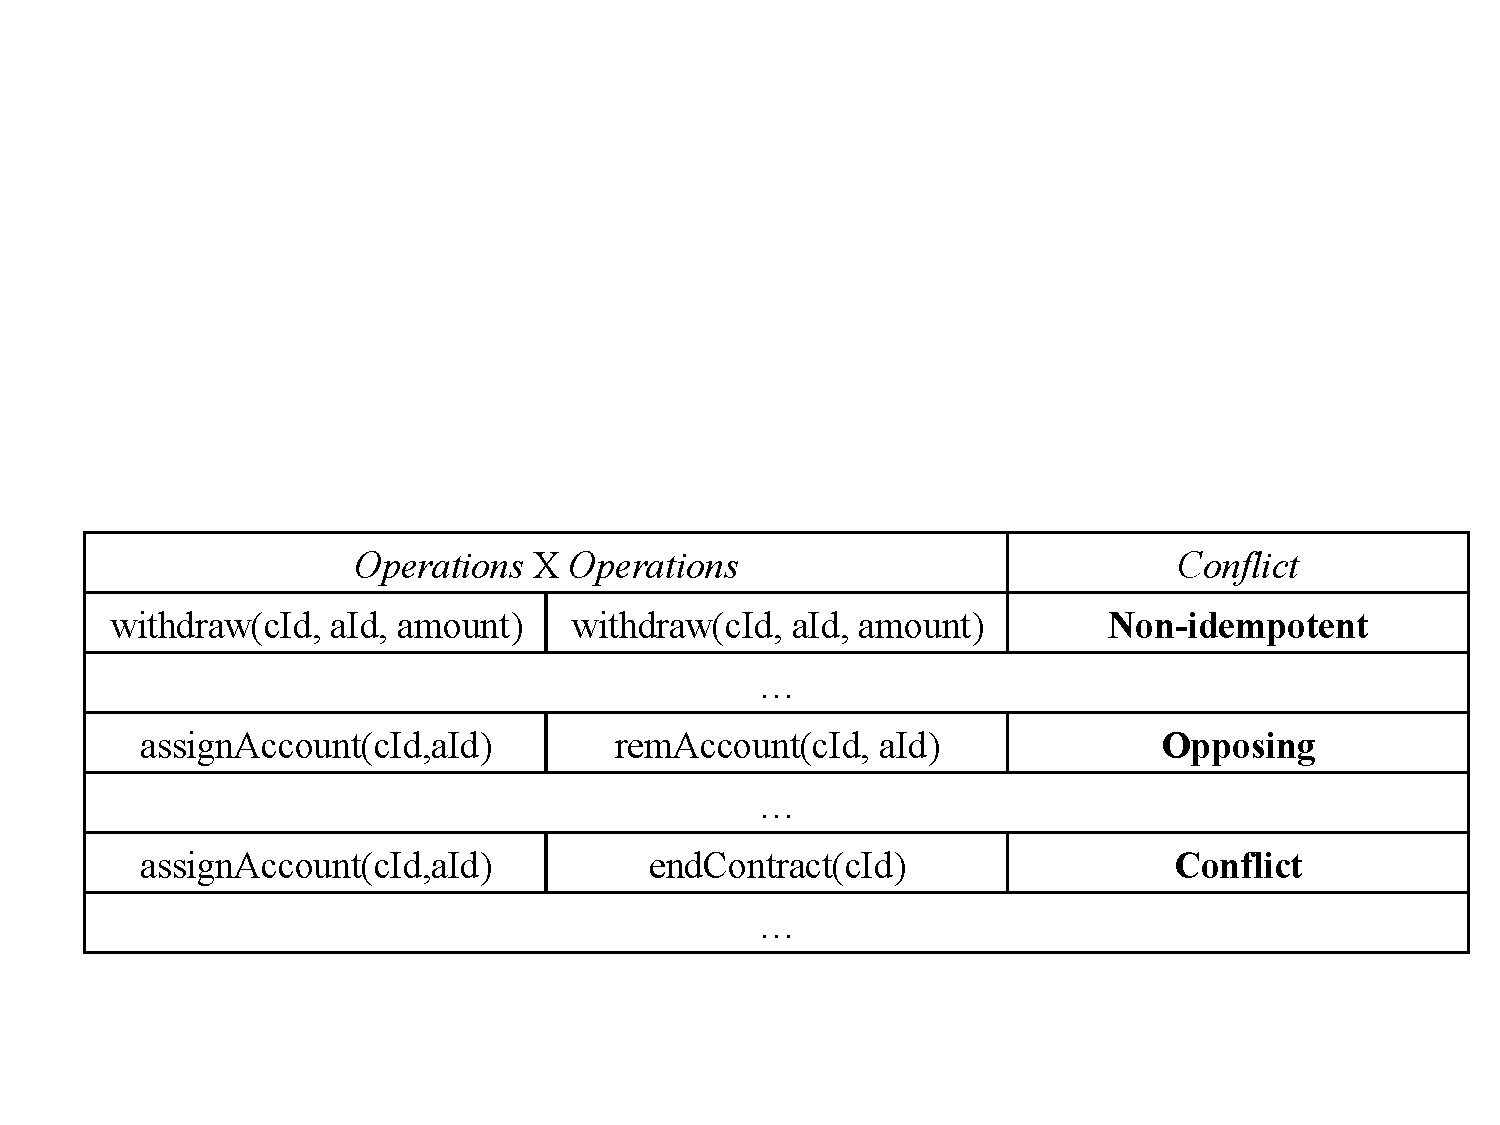
\includegraphics[width=\textwidth]{figures/conflict-table-cropped.pdf}
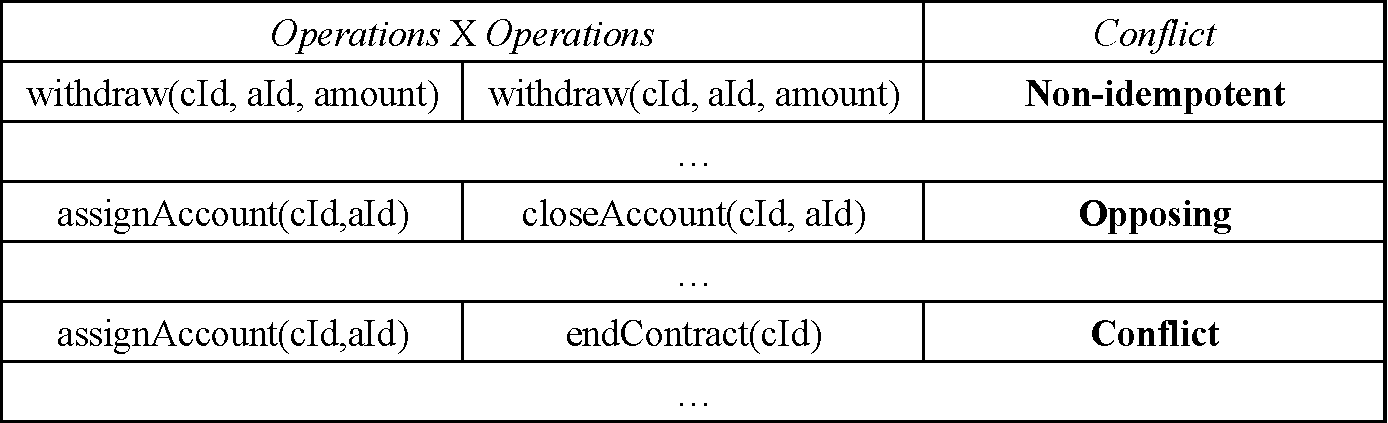
\includegraphics[bb=0 0 260 200]{conflict-table-cropped.pdf}
\label{fig:code-conflicts}
}
\end{minipage}
\caption{Bank application specification and analysis results.}
\end{figure}

\subsection{Analysis}
The analysis checks which are the shadow operations
whose concurrent execution might produce a
database state that is invalid with respect to the declared invariants.
Conceptually, for each pair of operations and for every valid state where
these operation can execute, the algorithm verifies if the execution of both
operations will lead to a state that is not valid according to the invariants
of the application.
%operations will lead to an invalid state where some application invariant
%does not hold.
%If this is the case, the concurrent execution of these operations can lead to
%an invariant violation.
Obviously, checking every pair of operations in every valid state
exhaustively is unfeasible. Instead, our algorithm relies in the
Z3 satisfiability modulo theory (SMT) solver to perform this verification
efficiently.
A full description of the algorithm is given in our prior publication~\cite{Balegas2015Indigo}.

%In an extension to our work, Gotsman et. al.~\cite{GotsmanConsistencyReason}
%prove that testing pairs of operations is sufficient for detecting if two
%operations might violate a defined invariant when executed concurrently.


%In order to do that, we use the Z3 satisfiability modulo theory (SMT) solver,
%to check, for every pair of shadow operations in the workload, $op_{i}, op_{j}$, if:
%\begin{itemize}
%    \item The execution of each operation produces a set of effects,
%        $E(op_{i})$ and $E(op_{j})$, that maintain the application invariants
%        when applied to the database individually.
%    \item There is a set of states $S$, in which both operations
%    		  $op_{i}, op_{j}$ can be applied together, i.e., that satisfy
%              the pre-conditions of both operations.
%    \item Both operation are invariant-safe, meaning that the effects of both operations
%        applied to all possible states $s_{i} \in S$ produces a new state
%        $s_{i} \cdot E(op_{i}) \cdot E(op_{j})$ that preserves the invariant.
%        Otherwise, the pair of operations is signaled as conflicting and the
%        reason is presented to the programmer.
%\end{itemize}

Figure~\ref{fig:code-conflicts} summarizes the conflicts in the example
of Figure~\ref{fig:code-snippet}:
two concurrent successful withdrawals might make the balance negative
(non-idempotence);
assigning and removing an account concurrently for the same user might leave
the system in an inconsistent state, because each shadow operation writes different
values for the predicate $userAccount(cId, aId)$ (opposing post-conditions);
and finally, the pair $createAccount(cId,$ $ aId)$ and $endContract(cId)$ might
violate the integrity constraint of line 3, because a new account is being
added to a user that is ending a contract with the bank.

%In the next section, we discuss how to address each of these conflicts
%efficiently.


%%The analysis algorithm checks which are the shadow operations
%%whose concurrent execution might produce a
%%database state that is invalid with respect to the declared invariants.
%%In order to do that, we use the Z3 satisfiability modulo theory (SMT) solver,
%%to check, for every pair of shadow operations in the workload, $op_{i}, op_{j}$, if:
%%\begin{itemize}
%%    \item The execution of each operation produces a set of effects,
%%        $E(op_{i})$ and $E(op_{j})$, that maintain the application invariants
%%        when applied to the database individually.
%%    \item There is a set of states $S$, in which both operations
%%    		  $op_{i}, op_{j}$ can be applied together, i.e., that satisfy
%%              the pre-conditions of both operations.
%%    \item Both operation are invariant-safe, meaning that the effects of both operations
%%        applied to all possible states $s_{i} \in S$ produces a new state
%%        $s_{i} \cdot E(op_{i}) \cdot E(op_{j})$ that preserves the invariant.
%%        Otherwise, the pair of operations is signaled as conflicting and the
%%        reason is presented to the programmer.
%%\end{itemize}
%%
%%A full description of the algorithm is given in our prior publication~\cite{Balegas2015Indigo}, and,
%%in a related piece of work~\cite{GotsmanConsistencyReason}, the authors prove that testing pairs of
%%operations is sufficient for detecting if two operations might violate a defined
%%invariant when executed concurrently.
%%
%%Figure~\ref{fig:code-conflicts} summarizes the conflicts in the example:
%%two concurrent successful withdraw shadow operations might make the balance negative
%%(non-idempotence);
%%assigning and removing an account concurrently for the same user might leave
%%the system in an inconsistent state, because each shadow operation writes different
%%values for the predicate $userAccount(cId, aId)$ (opposing post-conditions);
%%and finally, the pair $createAccount(cId,$ $ aId)$ and $endContract(cId)$ might
%%violate the integrity constraint of line 3, because a new account is being
%%added to a user that is ending its contract with the bank.
%%
%%%In the next section, we discuss how to address each of these conflicts
%%%efficiently.

\subsection{Code instrumentation}
After identifying which operations can lead to conflicts, the programmer
must instrument the application to avoid them.

Some conflicts can be handled by simply relying on CRDTs to automatically solve
them.
For example, our analysis can report that operations have 
opposing post-conditions: e.g., operations {\tt assignAccout} and {\tt remAccount}
assign the value \textit{true} and \textit{false} to predicate $userAccount(cId, aId)$.
In this situation, the programmer can choose a preferred value for the
predicate and use a CRDT that automatically implements the selected
decision\footnote{In our
experience, boolean predicates can be implemented using Set CRDTs with
add-wins and remove-wins policies to enforce that the corresponding 
predicate becomes true or false
respectively.}.

Other conflicts must be handled by restricting the concurrent execution of 
operations that can cause invariants to be broken. To this end, we provide a set 
of specialized reservation-based concurrency control mechanisms.

For conflicts on numeric invariants, like the one that withdraw causes,
% with the invariant that specifies that the balance should be non-negative, 
we support an escrow reservation for allowing some decrements of numeric 
values to execute without coordination.
In an escrow reservation, each replica is assigned a budget of decrements,
based on the initial value of the data.
In our example, when a replica receives a withdraw request, if the local 
budget is sufficient, the generator operation executes immediately 
without coordination, generating a shadow operation that decrements 
the balance.
This local execution is safe, guaranteeing that the invariant still holds
after executing all concurrent operations, because the sum 
of the budgets of all replicas is equal to the value of the initial value.
If the local budget is not enough to satisfy the request, the replica needs to
contact remote replicas to increase its budget, until it can satisfy the request.
If that is not possible, because there are not enough resources globally,
then the generator operation fails, generating no shadow operation.

For conflicts on generic invariants, we include a multi-value lock 
reservation. This lock can be in one of the following three states: 
(1) shared forbid, giving the shared right to forbid some action to occur; 
(2) shared allow, giving the shared right to allow some action to occur; 
(3) exclusive allow, giving the exclusive right to execute some action.
The idea is that, for a conflicting pair of operations, $(o_1,o_2)$, 
the lock will be associated with the execution of one of the operations, 
say $o_1$.
To execute $o_1$, a replica must hold the lock in the shared allow mode.
This right can be shared by multiple replicas.
To execute $o_2$, a replica must hold the lock in the shared forbid mode.
As before, when executing the generator operation, if the replica already
holds the necessary locks (in the required mode to execute the operation), 
it can execute locally and generate the corresponding shadow operation.
If not, it must contact other replicas to obtain the necessary locks.

Besides these two locks, we also proposed other locks that can
efficiently restrict the concurrent execution of operations that conflict 
in other types of invariants, including conditions on the number of elements
that satisfy a given condition and disjunctions.
In a related work, Gotsman et. al.~\cite{GotsmanConsistencyReason}
have shown how to prove that a given set of locks is sufficient
for maintaining invariants.




%%For numerical conflicts, like the one in the $withdraw(cId, aId, amount)$, we
%%provide the bounded counter CRDT~\cite{Balegas2015Counter}, which assigns to 
%%each replica a budget of decrement operations that each replica can execute.
%%When a replica receives a withdraw request, if the local budget is sufficient
%%to satisfy it, the generator operation executes immediately without coordination.
%%The local execution of the generator operation is safe because the sum of the budgets of
%%each replica is equal to the value of the counter.
%%If the local budget is not enough to satisfy the request, the replica needs to
%%contact remote peers to increase its budget, until it allows to satisfy the request.
%%If that is not possible, because there are not enough resources globally,
%%then the generator operation can fall back to safely going through the failed path,
%%which generates an invariant safe shadow operation---no-op.%no effects that might break invariants.
%%
%%For the second conflict reported by the analysis, the shadow operations have
%%opposing post-conditions: the value \textit{true} and \textit{false} are
%%assigned to the predicate $userAccount(cId, aId)$.
%%In this situation, the programmer must choose a preferred value for that
%%predicate.
%%In order to do so, the programmer must switch the data type implementing this
%%predicate to a CRDT and use the desired convergence policy~\footnote{In our
%%experience, boolean predicates can be implemented using Set CRDTs and
%%add-wins/remove-wins policies to enforce that the corresponding predicate becomes true/false
%%respectively.}
%%
%%When there is no conflict resolution mechanism for a specific type of invariant violations,
%%the programmer can control the execution of conflicting operations with CRDT tokens.
%%The idea of these tokens is that, for a conflicting pair of shadow operations, the replica
%%must hold a token to execute one of the corresponding generator operations.
%%The token only allows one of the corresponding generator operations to execute at a time,
%%the other is forbidden.
%%The token can act as a mutex, or multiple replicas can hold a piece of it to
%%execute the allowed generator operation concurrently with other peers.
%%When some replica needs to execute the generator operation that is being forbidden by the
%%token, it must coordinate with remote peers to revoke any permissions to
%%execute the current generator operation, and with this revocation they
%%incorporate all the shadow operations from the remote sites that still had
%%not been locally executed.
%%The runtime system must use some policy to ensure that all replicas eventually
%%satisfy their requests.




%\subsection{Comparison to RedBlue consistency}


